\subsection{Intensity Transformations in CryptoImg}
A paper published in 2009 by Ziad, et al. implements privacy-preserving image processing using \textit{CryptoImg}, a library for the Open Source Computer Vision Library (OpenCV)~\cite{bradski_opencv_2000} which implements various homomorphic encryption and image processing routines using the Paillier homomorphic cryptosystem~\cite{ziad_cryptoimg:_2016}. The \textit{CryptoImg} library assumed a client-server model wherein a client requests image processing operations from a server. A client first encrypts a digital image and sends the image securely to a server, which then operates on the encrypted image without revealing its contents. The resulting image is sent back to the client, which decrypts the image to recover the desired output.
\begin{figure}[!ht]
    \centering
    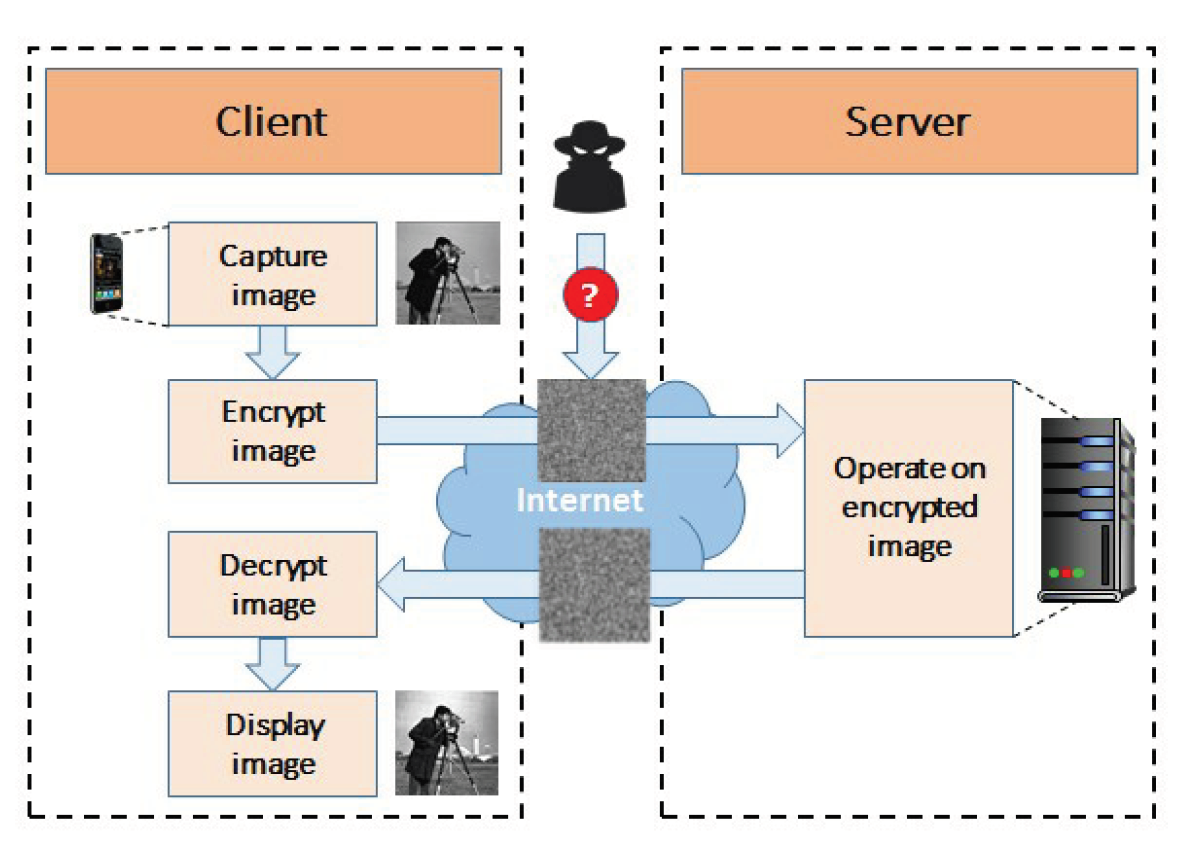
\includegraphics[width=0.4\textwidth]{figures/ClientServerModel.png}
    \caption{Architecture used by \textit{CryptoImg}, from \cite{ziad_cryptoimg:_2016}}
    \label{fig:clientserver}
\end{figure}

An intensity transformation on a digital image $R$ can be defined as a function $T$ which is applied to every pixel $r$ in $R$. Table \ref{tab:imageoperation_summary} shows common image intensity transformations~\cite{gonzalez_digital_2008}. 
The \textit{CryptoImg} library implemented two types of intensity transformations: image negation and brightness control, which are both linear transformations. 
In this study, we consider two common non-linear transformations. the logarithm transformation and power-law transformation~\cite{gonzalez_digital_2008}, seen in Table \ref{tab:imageoperation_summary}.

% The \textit{CryptoImg} library implemented the following image processing operations: image negation, brightness adjustment, spatial filters (for noise reduction, edge detection and sharpening), morphological operations, and histogram equalization. 


% For image negation and spatial filters, the protocols specified by \textit{CryptoImg} allow all image processing operations to be performed on the server. However, due to limitations in the Paillier cryptosystem, the protocols presented for morphological operations and histogram equalization require both the client and the server to perform image processing calculations, although the server performs a significant portion of the processing.

% Ziad, et al. also showed experimental results establishing the relatively slow performance of image operations under a homomorphic cryptosystem. For instance, while sharpening and applying a Sobel filter each take less than a second when applied to a $512\times 512$ plaintext image, when applied to an encrypted image, sharpening required at least 238.257 seconds, and applying the Sobel filter required at least 147.567 seconds \cite{ziad_cryptoimg:_2016}.


% We now discuss several limitations in the \textit{CryptoImg} study which we focus on for our research. First, the \textit{CryptoImg} library was limited in the image intensity transformations it implemented. We propose additional protocols to support more computationally intensive intensity transformations.
% Second, the \textit{CryptoImg} library only considered the Paillier cryptosystem. We consider testing the performance of other homomorphic cryptosystems, which differ in their processing time and supported operations.

% Convert to single table
\begin{table}[ht]
	\caption{Summary of intensity transformations}
	\label{tab:imageoperation_summary}
    \begin{tabular}{
        p{\dimexpr 0.65\linewidth-2\tabcolsep}
        p{\dimexpr 0.35\linewidth-2\tabcolsep}}
		\toprule
		Operation & Transformation\\
        \midrule
            Image negation &
            $T\left(r\right) = L-1-r$
            \\
            Brightness adjustment transformation with parameter $v$ &
            $T\left(r\right) = r+v$
            \\
            Logarithm transformation with parameter $c$ &
            $T\left(r\right) = c \log\left(1 + r\right)$\\
            Power-law transformation with parameters $c$ and $\gamma$, where $c>0$ and $\gamma > 0$&
            $T\left(r\right) = c r^{\gamma}$\\
	    \bottomrule
    \end{tabular}
\end{table}
% We represent a digital image $R$ as an $M \times N$ matrix of pixel intensity values, each value in the range $\left[0, L-1\right]$, for some positive integer $L$. We denote with $R(x,y)$ the entry at the $x$th row and $y$th column of a matrix $R$.
The logarithm transformation is used to enhance dark pixels or increase the dark details of an image by mapping low intensity values to a wider range of values. A power-law transformation can calibrate the operation of many image capture and output devices such as cameras, printers and displays in a process called \textit{gamma correction}~\cite{gonzalez_digital_2008}. Both of these transformation can be used in intensity normalization \cite{oravec_illumination_2010}, which is used in some facial recognition algorithms to account for differences in lighting which make facial recognition difficult.

To implement non-linear intensity transformations in a privacy--preserving system, it is necessary to evaluate logarithm and exponential functions using closed--form approximations, since the arguments of the functions are unknown. An applicable approximation for the logarithm, found in \cite{pcsc-paper}, is
% TODO: HOW ABOUT BGV
\begin{align}\label{eq:optimal_log_approximation}
	\begin{split}
		&\log\left(1+x\right) \approx \frac{a(x)}{b(x)} + \log{16} ,
	\end{split}
\end{align}
where
\begin{align*}
	\begin{split}
	a(x) &= 137x^5 + 26685x^4 + 617370x^3 - 6498630x^2 \\
	&- 121239315x - 257804775\\
	b(x) &= 30(x^5 + 405x^4 + 27210x^3 + 488810x^2 + 2536005x \\
	&+ 3122577).
	\end{split}
\end{align*}
This approximation can be computed under a homomorphic cryptosystem which supports floating-point operations by precomputing the value of $\log{16}$ in the plaintext domain.
% \begin{align}\label{eq:optimal_log_approximation}
% 	\begin{split}
% 		&\log\left(1+x\right) \\
% 		&\approx \frac{137x^5 + 26685x^4 + 617370x^3 - 6498630x^2 - 121239315x - 257804775}
% 		{30(x^5 + 405x^4 + 27210x^3 + 488810x^2 + 2536005x + 3122577)}\\
% 		&+ \log{16}.
% 	\end{split}
% \end{align}

% \subsubsection{Power-Law Transformation}
To apply the power-law transformation we can use partial sums of the infinite series,
\begin{align} \label{eq:power_approximation}
	x^\gamma &= \sum_{n=0}^{\infty}{\frac{(\gamma\log{x})^n}{n!}},
\end{align}
which relies on the logarithm function.
For the implementation of the power-law transformation for this paper, a partial sum consisting of the first five terms of the infinite series were used.
